\chapter{Uplift Modelling}
\label{ch-uplift}


This chapter is based mainly on Ref.\cite{scikit-uplift}.
Ref.\cite{scikit-uplift} is the github repo for
the excellent open source Python package {\tt scikit-uplift}.
As its name implies, this package is
integrated with the Python libraries {\tt scikit}, in especially
the AI package {\tt scikit-learn} .
 {\tt scikit-uplift} contains a great tutorial 
 on uplift modelling
 done with its software. It also contains about half a dozen
jupyter notebooks illustrating the usage
of its software for various datasets which it includes. I've also created
my own repo called {\tt uplift\_rocket}
(Ref.\cite{uplift_rocket})
where I give examples of the use of
the {\tt scikit-uplift}  software.



\begin{figure}[h!]
$$\begin{array}{ccc}
\xymatrix{
&\rvx\ar[dr]
\\
\rvd\ar[rr]
&&\rvy
}
&\quad&
\xymatrix{
&\rvx\ar[dr]
\\
\rvy_0\ar[rr]
&&\rvy
}
\\
(a) &\quad & (b)
\end{array}
$$
\caption{Bnets for Uplift Modelling (UM). 
Bnet $(a)$ is for an RCT experiment measuring Uplift and Bnet $(b)$ is for one measuring Uplift2. 
 Since we assume an RCT, the arrows $\rvx\rarrow \rvd$ 
and $\rvx\rarrow \rvy_0$ have been amputated (i.e., removed). This is equivalent to assuming that $P(d|x)=P(d)$ and
$P(y_0|x)=P(y_0)$.
}
\label{fig-up-bnet}
\end{figure}


{\bf Uphill Modelling} (UM) (a.k.a., {\bf Uplift Marketing})
is an experiment that performs an
RCT (Randomized Controlled Trial) and additional steps. It 
entails performing an
RCT  and 
 calculating  the \qt{Uplift} or \qt{Uplift2} for that  RCT.
 \footnote{Uplift and Uplift2 to be defined later.}
From that, UM builds a classifier that opines whether individuals are
persuadable or not. UM also plots something called a Qini curve that predicts
what fraction of the population is persuadable. 

UM is often used to identify which 
customers are more likely to be persuaded to buy a
product, or to identify which voters are more
likely to be persuaded to vote for a target political candidate.
Once marketers or election campaigners know this, they can concentrate their limited resources only on the persuadables. Note, however, that UM is not only useful
to marketers and election campaigners. For example, it could be used to prioritize organ transplant recipients. 
More generally, it can be used to
prioritize the allocation of 
a scarce resource.

Fig.\ref{fig-up-bnet} shows bnets for 2 experiments. Bnet $(a)$\footnote{
Note that bnet \ref{fig-up-bnet}$(a)$ 
is the bnet for Rubin's theory of 
Potential Outcomes (PO).
PO, which is
discussed in Chapter \ref{ch-pot-out},
 is a subset
of Pearl's Causal Inference.
Besides UM, other  applications of PO theory
that are discussed in this book 
are: Regression Discontinuity (Chapter \ref{ch-reg-dis}),
Difference-in-Differences (Chapter \ref{ch-did})
and Synthetic Controls (Chapter \ref{ch-syn-con}).} is for an RCT experiment measuring 
Uplift and Bnet $(b)$ is for one measuring Uplift2. 
The node variables of bnets Fig.\ref{fig-up-bnet}
$(a)$ and $(b)$
are defined as follows:

$x=(x_0, x_1,\dots, x_{n-1})$ is an $n$ dimensional 
vector of features $x_i$. If any of the $x_i$
is a priori continuous, we will
assume it has  been binned into
a finite number of bins.
Let $val(\rvx)$ be the finite set of  all feature vectors.

$\rvd\in\bool$ is the {\bf treatment dose} or just treatment for short. For campaigners, it equals 1 iff voter receives
a brochure (which
we will call the {\bf intervention}
or {\bf treatment}) trying to convince him/her to vote 
for the target  candidate. The cohort with $\rvd=0$ is called the {\bf control group}. The one with $\rvd=1$ is called the {\bf treated group}.
The intervention occurs between times $t_0$ and $t_1$
where $t_0<t_1$.

$\rvy_0=\rvy_{t_0}\in \bool$ is the 
{\bf pre-treatment response}. For campaigners, whether a voter would
vote for a candidate at time $t_0$.

$\rvy=\rvy_{t_1}\in \bool$
is {\bf treatment response or outcome}. For campaigners, whether a voter would
vote for a candidate at time $t_1$. 

Although we are referring to bnets $(a)$
and $(b)$ as 2 different experiments, they can be done
simultaneously. Enacting
bnet $(a)$ requires splitting the initial 
randomized population into two equal parts:
the control group and the treated group.
The control group is not treated (its members do
not receive the persuasive brochure or treatment). On the other hand, enacting bnet $(b)$ requires
sending all customers, before and after treatment, both (1) a brochure/treatment,
and  (2) a questionnaire/survey asking them who they are voting for.
Hence, one can use the treated group of
bnet $(a)$ as the full cohort of bnet $(b)$.

Note that bnet $(a)$, 
\beq
P(y, d, x) = P(y|d,x)P(d)P(x)
\eeq
and for bnet $(b)$,
\beq
P(y, y_0, x) = P(y|y_0,x)P(y_0)P(x)
\eeq

Usually, $P(d) = \frac{1}{2}$.

Let us denote each {\bf customer} (i.e., {\bf voter}, {\bf participant},  {\bf sample}) 
by $\s$,
where 
\beq\s\in \Sigma=\{0,1,2, \ldots, nsam-1\}
\eeq

\subsection{Uplift definition}


We will call 

\beq
\delta(x)=
P(\rvy=1|\rvd=1, \rvx=x) -
P(\rvy=1|\rvd=0, \rvx=x)
\eeq
the {\bf uplift for stratum $x$}.
If $x=x^\s$, we can call it the {\bf uplift
for individual $\s$}.
Note that this identical to what 
we referred to in the chapter on PO theory (Chapter \ref{ch-po-out}) as: ATE (Average Treatment Effect) or
ACE (Average Causal Effect). ATE=ACE.\footnote{More precisely, this is
CATE (conditional ATE) or CACE (Conditional ACE),
$CATE= ATE_x$ and $ATE=\sum_x P(x)ATE_x$.} However, 
here we are applying it to 
the specialized scenario of an RCT. 


\subsection{Uplift2 definition}


We will call 

\beq
\delta^\s=
y^\s_{t_1}-y^\s_{t_0} = y^\s-y^\s_0
\eeq
the {\bf uplift2
for customer $\s$}.
Also, we will call

\beqa
\delta(x) &=& \sum_{y, y_0}(y - y_0)P(y, y_0|x)
\\
&=& 
\underbrace{\sum_{y}yP(y|x)}_{\av{\rvy}_x}
- 
\underbrace{\sum_{y_0}y_0P(y_0|x)}_{\av{\rvy_0}_x}
\label{eq-delta-x-def}
\eeqa
the {\bf uplift2 for stratum $x$}.
Note that $P(y_0|x)= P(y_0)$ by assumption so

\beq
\av{\rvy_0}_x = \av{\rvy_0}
\eeq
If $y, y_0\in \bool$,

\beq
\delta(x) = P(\rvy=1|x) - P(\rvy_0=1|x)
\eeq

Note that for Uplift2, we can refer
to either $\delta^\s$ or $\delta(x^\s)$ as
the Uplift2 for customer $\s$.
\subsection{UM customer types}
\label{sec-up-types}

\begin{figure}[h!]
\centering
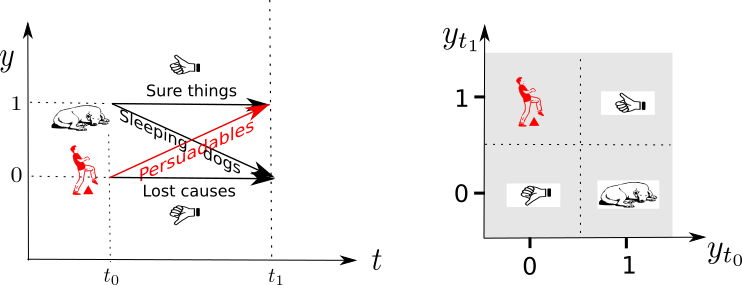
\includegraphics[width=6in]
{uplift/uplift-y-t-up.png}
\caption{UM-intervention
can be used to classify
all customers of the
population into 4 UM-types.
This figure 
assumes $y\in \bool$.
More generally, $y\in \RR$.
$t$ represents time. $t_0< t_1$.
This figure is for Uplift2. 
For Uplift replace $y_{t_0}$ by $d$.} 
\label{fig-uplift-y-t}
\end{figure}

As shown
in Fig.\ref{fig-uplift-y-t},
UM classifies customers
into 4 {\bf UM-types}: Persuadables, SureThings, LostCauses,
and SleepyDogs.
The UM-type
of a customer
depends on the changes 
that are induced on that customer
by an {\bf UM-intervention}.
\begin{itemize}
\item
For a {\bf Persuadable} customer,
$\delta(x^\s)>0$.
\item
For a {\bf SleepyDogs}
customer, $\delta(x^\s)< 0$.
\item
For a {\bf SureThings} customer,
 $\delta(x^\s)\approx 0$
and $y^\s_{t_0}=1$ for Uplift2
 (or $d=1$ for
Uplift).
\item
For a {\bf LostCauses} customer,
$\delta(x^\s)\approx 0$
and $y^\s_{t_0}=0$ for Uplift2
 (or $d=0$ for
Uplift).
\end{itemize}

\section{UM classifiers}
Chapter \ref{ch-meta-learners} on \qt{Meta-learners}

\begin{itemize}
\item {\bf S (Single)-learner}

\beq
\{(\s, x^\s,d^\s, \boxed{y^\s} ):\s\in \Sigma\}
\mlarr \haty(d,x), P(\rvy=1|d,x)
\eeq

\beq
\delta(x)= P(\rvy=1|\rvd=1, x)-P(\rvy=1|\rvd=0, x)
\eeq

\item {\bf T (Twin)-learner}

\beq
\{(\s, x^\s,d^\s=0, \boxed{y^\s} ):\s\in \Sigma\}
\mlarr \haty_0(x), P(\rvy=1|\rvd=0, x)
\eeq

\beq
\{(\s, x^\s,d^\s=1, \boxed{y^\s} ):\s\in \Sigma\}
\mlarr \haty_1(x), P(\rvy=1|\rvd=1, x)
\eeq

\beq
\delta(x)= P(\rvy=1|\rvd=1, x)
- P(\rvy=1|\rvd=0, x)
\eeq
\end{itemize}

\section{UM metrics and plots}
This section refers to Uplift.
All it results are valid for 
Uplift2 if we replace $d$ by $y_0$.





\begin{itemize}
\item {\bf Contingency Table}

Calculate $2\times 2$ table with cells $(d, y)$
where $d, y\in\bool$. The entry of cell
$(d,y)$ is the number of individuals $\s$
with $(d,y)=(d^\s, y^\s)$.

For example, suppose $d^\s=[0,0,1]$
and $y^\s=[1,1,0]$. Then $(d^\s,y^\s)= (0,1), (0,1), (1,0)$
so the contingency table is

\begin{table}[h!]
\begin{tabular}{|l|l|l|}
\hline
$d \backslash y$ & \cellcolor[HTML]{FFFFC7}0 & \cellcolor[HTML]{FFFFC7}1 \\ \hline
\cellcolor[HTML]{FFFFC7}0 & 0 & 2 \\ \hline
\cellcolor[HTML]{FFFFC7}1 & 1 & 0 \\ \hline
\end{tabular}
\caption{Contingency table example}
\label{tab-con-tab}
\end{table}

\item {\bf Uplift by percentile (i.e., by bin) plot}

\begin{itemize}[\checkmark]
\item Assume the population is ordered in decreasing 
order of Uplift. Hence,

\beq \delta(x^1)\geq \delta(x^2)\geq \delta(x^3)\geq \cdots
\eeq
\item Bin this sequence of uplifts into bins with $n_C$ individuals
for the control group bins 
and $n_T$ for the treated group bins.
\item Plot bin label versus average uplift in bin.
Alternatively, plot bin label versus average of response
in treated group minus average of response in control group.
Plot can be a bar graph or a continuous curve

\end{itemize}

\item {\bf percentile bin vs bin av. uplift plot}
\item {\bf Qini curve}

Assume the population is ordered in decreasing 
order of Uplift. Hence,

\beq \delta(x^1)\geq \delta(x^2)\geq \delta(x^3)\geq\cdots\eeq
Let 

\beq S_{\Delta} = \{\s:\delta(x^\s) \geq \Delta\}\eeq
A Qini curve is a
 plot of $(X_\Delta, Y_\Delta)$ for all $\Delta>0$,
where

\beq
X_\Delta = |S_{\Delta}|, \quad
Y_\Delta= \sum_{\s\in S_{\Delta}}\delta(x^\s)
\eeq
 As $\Delta$ decreases, a Qini curve rises fast at first, and then its slope decreases,
 until
at some threshold slope value $c_0$, the slope is 
considered as too small to care. No marketing resources are
directed towards
customers with slope beyond that point.

\end{itemize}


\begin{figure}[h!]
\centering
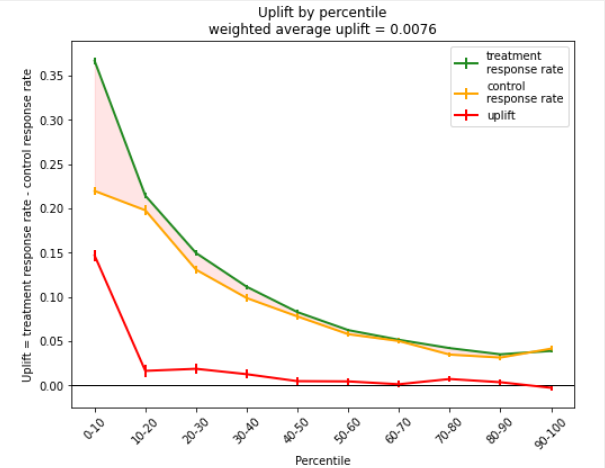
\includegraphics[width=5in]
{uplift/line-uplift-binned.png}
\caption{Mount Vesuvius and Bay of Naples 
(from Ref.\cite{scikit-uplift})}
\label{fig-line-up-bin}
\end{figure}

\begin{figure}[h!]
\centering
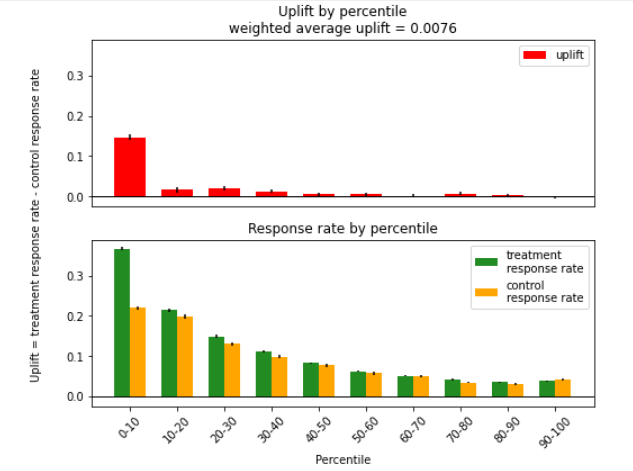
\includegraphics[width=5in]
{uplift/bar-uplift-binned.png}
\caption{Mount Vesuvius and Bay of Naples 
(from Ref.\cite{scikit-uplift})}
\label{fig-bar-up-bin}
\end{figure}

\begin{figure}[h!]
\centering
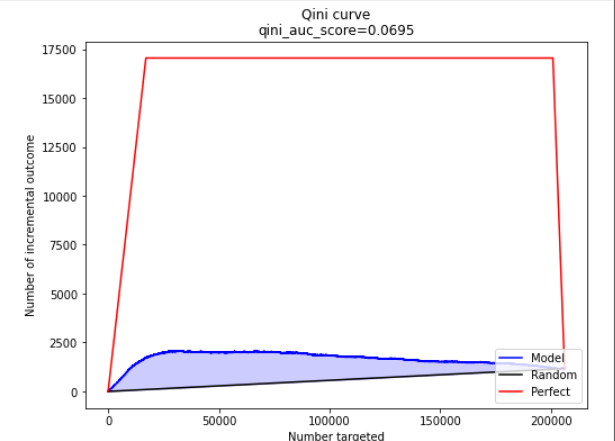
\includegraphics[width=5in]
{uplift/qini.png}
\caption{Mount Vesuvius and Bay of Naples 
(from Ref.\cite{scikit-uplift})}
\label{fig-qini}
\end{figure}



